\documentclass[12pt,a4paper]{article}

% ---------- Packages ----------
\usepackage[utf8]{inputenc}
\usepackage[T1]{fontenc}
\usepackage{lmodern} % Better font rendering
\usepackage{geometry} % Page layout
\geometry{margin=1in}
\usepackage{setspace} % Line spacing
\onehalfspacing
\usepackage{hyperref} % Clickable links
\usepackage{titlesec} % Custom section formatting
\usepackage{enumitem} % Better lists
\usepackage{amsmath, amssymb, amsthm} % Math
\usepackage{tcolorbox} % For highlighted boxes
\usepackage{graphicx} % For images/figures
\usepackage{booktabs} % Better tables
\usepackage{parskip}

% ---------- Section Formatting ----------
\titleformat{\section}{\large\bfseries}{\thesection}{1em}{}
\titleformat{\subsection}{\normalsize\bfseries}{\thesubsection}{1em}{}
\titleformat{\subsubsection}{\normalsize\itshape}{\thesubsubsection}{1em}{}

% ---------- Custom Environments ----------
\newtcolorbox{definitionbox}{
  colback=blue!5!white,
  colframe=blue!50!black,
  title=Definition,
  fonttitle=\bfseries
}

\newtcolorbox{examplebox}{
  colback=green!5!white,
  colframe=green!50!black,
  title=Example,
  fonttitle=\bfseries
}

\newtcolorbox{notebox}{
  colback=yellow!10!white,
  colframe=yellow!50!black,
  title=Note,
  fonttitle=\bfseries
}

% ---------- Document ----------
\begin{document}

\begin{center}
    {\LARGE \textbf{AI Notes}} \\
    \vspace{0.5em}
    {\large Notes on \textit{Chapter 2: Data, Measurements, and Data Preprocessing}} \\
    \vspace{0.5em}
    \textbf{Author: Abdullah Yassine} \\
    \today
\end{center}

\tableofcontents
\newpage

% ---------- Example Structure ----------
\section{Data Types}
\textbf{Data object} is an entity. Objects can be things like employees at a company, customers at a business, and so on. The \textbf{attributes} that describe those objects are a feature of the object. They describe something of the object. Salary is an attribute of an employee, the number of items bought is an attribute of a customer, and so on.

Attributes can have different ranges of values. We explore them here.

\subsection{Nominal attributes}

\textbf{Nominal attributes} are \textit{names of things}. They cannot be ordered, but are categorized. Things like the colors of an eye, types of t-shirts, and so on. 

Those attributes can also be turned into numbers, like 0 for black, 1 for red, and so on. But mathematical operations on these numbers are meaningless. It does not mean anything when you take the mean for example. You can take the mode which we take about later.

\subsection{Binary attributes}

A \textbf{binary attribute} only have two values, 0 or 1, or True or False. 

A binary attribte can be \textbf{symmetric} if there is no preference on who gets the 1 or 0, like male or female.

An \textbf{assymetric} binary attribute is where it's not equally important. Like \textit{positive} or \textit{negative} of a disease.

\subsection{Ordinal attributes}

An \textbf{ordinal attribute} is where you can rank them, but the magnitude of difference between successive values aren't known. This is things like small, medium, or large, but we can't tell how much larger a large is from a medium. Because you can order them, we can take the mode and median, but not the mean. 

\subsection{Numeric attributes}

A \textbf{numeric attribute} is measurable quantity.

\textbf{Interval-scaled attributes} are measured on equal-sized scale. They can be zero, positive, or negative, and they do have an order. We can also quantify the difference between values here. For example, temperates of 10 and 50 Celsius can have a difference of 40, but you cannot have ratios here or that they don't have meaning.

\textbf{Ratio-scaled attributes} have an inherent zero-point scale, so you can take ratios and they do have meaning. If you take temperature in Kelvin, this is where this comes. Other things include counts of things like \textit{years of experience} or \textit{number of words} are ratio-scaled.


\subsection{Discrete vs. continous attributes}

A \textbf{discrete attribute} can have limited number of values or can be countably infinite. It can numeric or otherwise. Things like \textit{color of eye}, \textit{sizes of drinks}, and so on. They can numeric, for example, 0 and 1 for binary attributes. Countably infinite just means the range of values can be infinite, but those values can be "listed" one by one, like \textit{customer\_id} or zip codes.

\textbf{Continous} is just infinite, if it's not discrete.


\section{Statistic of Data}

\subsection{Measuring the central tendancy}

Central tendancy is what measures the middle of things so we can have a picture of the middle of the distribution. First, we have the \textbf{mean}: $$\bar{x}=\frac{\sum_{i=1}^{N} x_i}{N} = \frac{x_1 + x_2 + \dots + x_n}{N}$$

Sometimes, we want to give weights to some of the elements signifying their importance. If so, we use the following \textbf{weighted average}: $$\bar{x}=\frac{\sum_{i=1}^{N} w_ix_i}{\sum_{i=1}^{N} w_i} = \frac{w_1x_1 + w_2x_2 + \dots + w_nx_n}{w_1 + w_2 + \dots + w_n}$$

Sometimes, the mean is not the best tool because it's very sensitive to outliers. We can use \textbf{trimmed mean} and just ignore those outliers.

The next tool we have is the \textbf{median} which is the value that seperates the left half from the right half given the list is ordered.

The next tool we have is \textbf{mode}, which is the value that occurs the most often in the distribution. Sometimes, a distribution can have multiple modes, so we call the distribution \textbf{multimodal}.

Another tool is the \textbf{midrange} which can be used to assess the central tendancy of the dataset. It's the average of the largest and smallest values of the list. Look at the following picture to see the difference between symmetric and asymmetric or skewed data:

\begin{figure}[h]
    \centering
    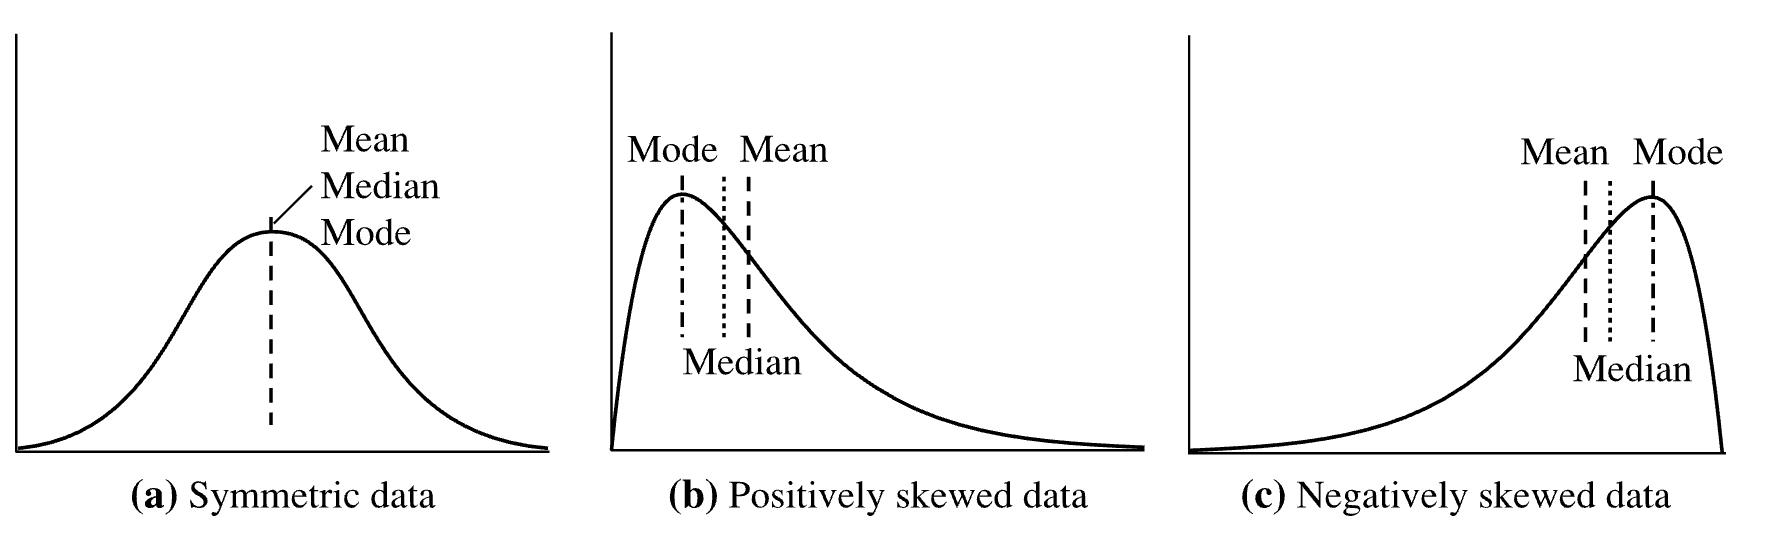
\includegraphics[width=0.7\textwidth]{images/image.png}
    \caption{Difference between symmetric and assymetric}
    \label{fig:example}
\end{figure}

\section{Measuring the Dispersion of Data}

We now try to measure the spread of data. We begin with \textbf{range}, which is the just the difference between the largest value and the smallest value in the set.

Then, we have \textbf{quantiles} which are points taken at regular intervals that essentially divide the set into equal parts. 

The 4-quantiles are the ones that divide the data set into four equal parts, they are also called \textbf{quartiles}. We also have the \textbf{percentiles} which divide the data into 100 equal-sized parts.

Back to the quartile, the \textbf{first quartile} is the 25\% percentile, which cuts off the lowest 25\%. You also have the \textbf{third quartile}, which cuts off the lowest 75\%. The distance between the first and third quartiles is simply the range of the middle half of the data. This is called \textbf{interquartile range} (IQR): $$\text{IQR} = \text{Q}_3 - \text{Q}_1$$ 

If the data set is odd, then you exclude the median element and divide up the set into the left half and the right half then calculate median again. If even, you must include them again and divide into left and right half while including them.

Another way of identifying \textbf{outliers} is to see if the suspected outlier is above $1.5 \times \text{IQR}$ of the third quartile or below the first quartile.

Thus, we have the \textbf{five-number summary} which consists of \textit{minimum} (smallest value), $Q_1$, median, $Q_3$, \textit{maximum}, and this is represented by \textbf{boxplots}.

Boxplots have following properties:
\begin{itemize}
    \item Ends of boxes is quartiles.
    \item Middle part is median.
    \item The lines are extended to the smallest and largest observations.
\end{itemize}

If outliers are beyond $1.5 \times \text{IQR}$, we draw them as points as individuals. When that happens, we draw the actual $1.5 \times \text{IQR}$ as well as the individual points:

\begin{figure}[h]
    \centering
    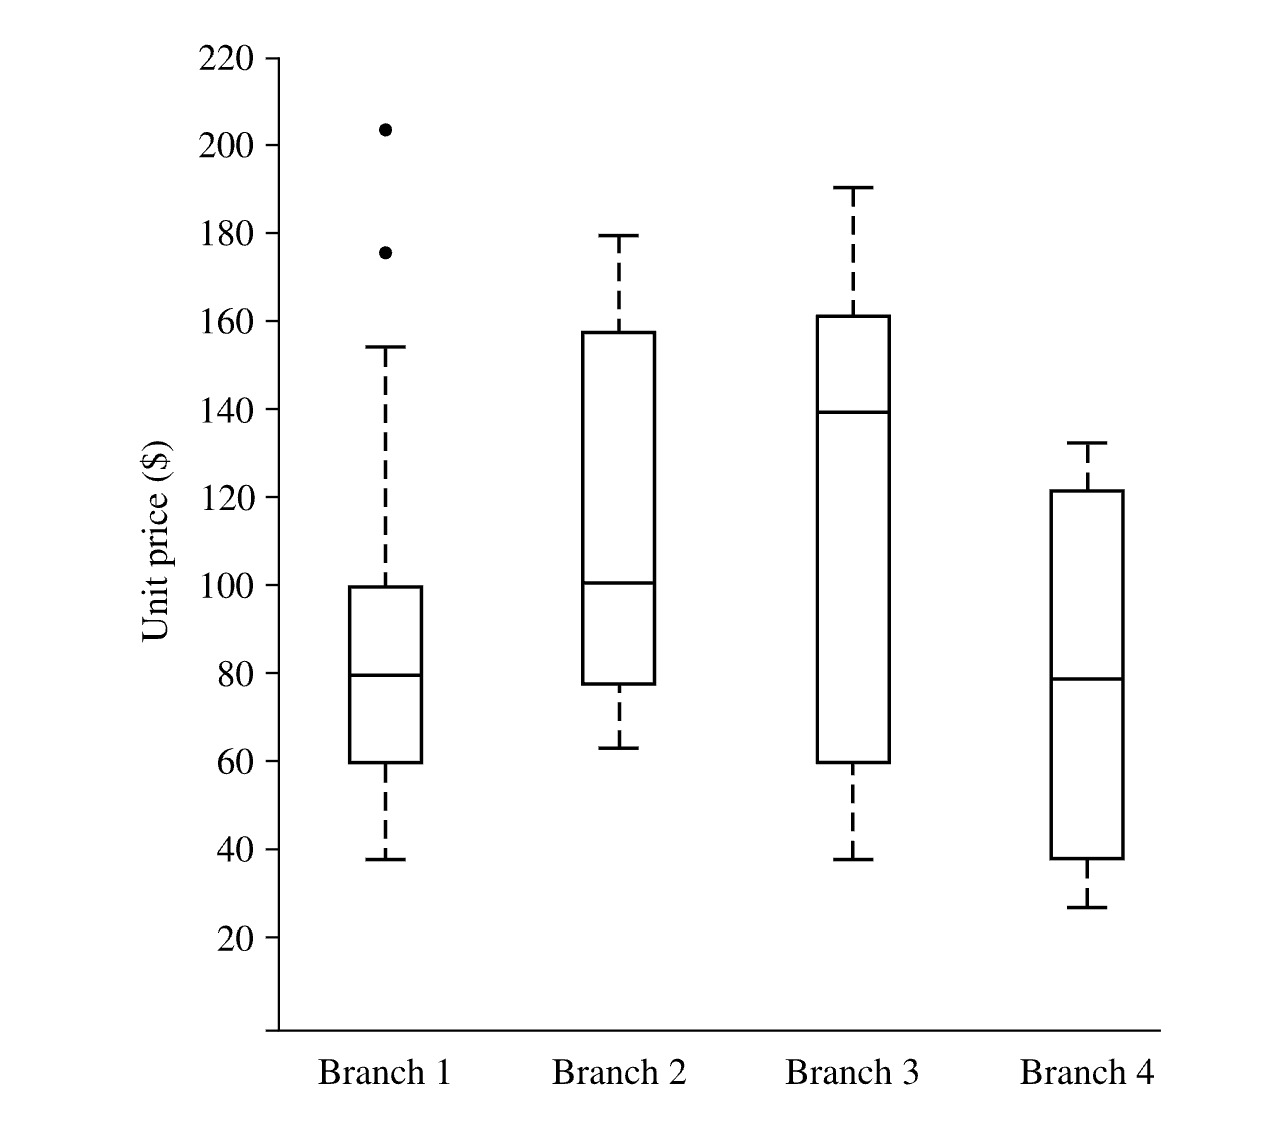
\includegraphics[width=0.7\textwidth]{images/image2.png}
    \caption{Example of boxplot}
    \label{fig:example1}
\end{figure}

\subsection{Variance and standard deviation}

\textbf{Variance} is calculated as following: $$\sigma^2 = \frac{1}{N}\sum_{i = 1}^{N} (x_i - \bar{x})^2 = \left(\frac{1}{N}\sum_{i = 1}^{N} x_i^2\right) - \bar{x}^2$$

\textbf{Standard deviation} ($\sigma$) is just the square of variance. SD is zero when there is no spread, otherwise it's positive.

\section{Covariance and Correlation Analysis}








\end{document}
